\section{Results and Discussion}\label{sec:Discussion}

If not otherwise specified, the results have been derived using the following parameters:
\begin{itemize}
	\item Harmonic oscillator frequency $\omega = 1$
	\item Coulomb interaction strength and shielding constants $\alpha = 1$, $\beta = 0$
	\item Metropolis step length $step\_length = 1$
	\item Number of Metropolis steps $steps = 20$
	\item Batch size of 500
	\item Training duration of 500 epochs
	\item Two layer DNN architecture with $32$ nodes each  
\end{itemize}


\subsection{Pure DNN Model for One Particle In Harmonic Oscillator}
\subsubsection{One Particle in 1D Harmonic Oscillator, Relu vs Tanh}

\begin{figure}[H]
	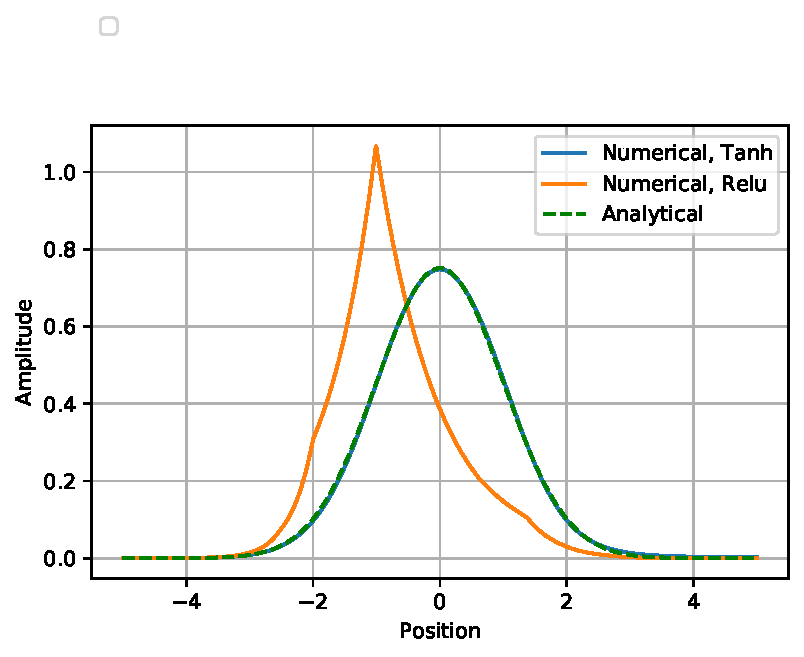
\includegraphics[]{figures/one_part_wavefunc.pdf}
	\caption{Wave function of particle in 1D harmonic oscillator, $\omega=1$, approximated using DNN with Tanh and ReLu activations, respectively. The Metropolis step length was set to $2$. The results are plotted against the analytical result}
	\label{fig:one_part_func}
\end{figure}

In figure \autoref{fig:one_part_func}, we see the result of training the DNN trial wave function on a single particle in a $1D$ harmonic oscillator. The Metropolis step length was set to $2$ to yield $\approx 50\%$ acceptance rate. Upon first exception, we see that the trial wave function using $ReLu$ as activation fails spectacularly in approximating the analytical result, while $Tanh$ produces a very close-lying approximation. 

\begin{figure}[H]
	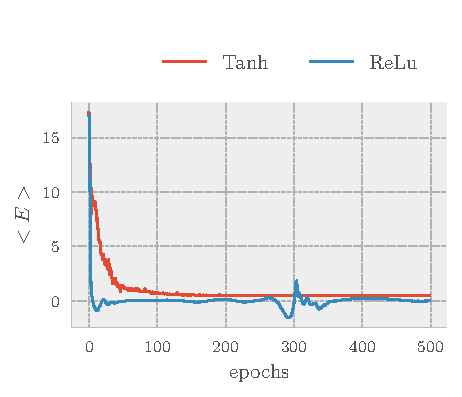
\includegraphics[]{figures/one_part_training1.pdf}
	\caption{Energy estimated from each batch during training of the $Tanh$ and $Relu$ model on one particle in 1D harmonic oscillator}
	\label{fig:one_part_training1}
\end{figure}

The minimization of $\langle E \rangle$ during training for the $ReLu$ and $Tanh$ model can be seen in \autoref{fig:one_part_training1}, and reveals even more serious problems with $ReLu$. While the energy of the $Tanh$ model smoothly decreases towards the analytical value of $E=0.5$, the energy of the $ReLu$ model varies wildly, even undercutting the analytical value. This is disastrous, as it violates the variational principle. 

\begin{figure}[H]
	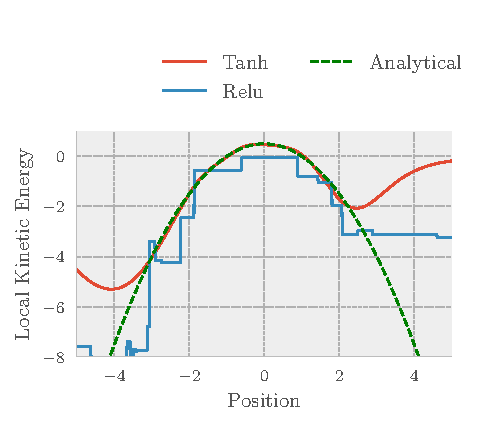
\includegraphics[]{figures/one_part_local_kinetic.pdf}
	\caption{Local kinetic energy of the $Tanh$ and $Relu$ model trained on one particle in $1D$ harmonic oscillator}
	\label{fig:one_part_local_kinetic}
\end{figure} 

\autoref{fig:one_part_local_kinetic} shows the local kinetic energy(the kinetic term entering the local energy) as a function of position for the $ReLu$ and $Tanh$ model. This is plotted against the analytical result. As can be seen, the local kinetic energy of $ReLu$ model is very ill-behaved, is most likely the cause of the violation of the variational principle. Since the local kinetic energy relies on the Laplacian of the trial wave function, the use of activation functions with discontinuous derivatives, such as $Relu$, appears to produce models which cannot approximate wave functions with appropriate curvature.

Further, \autoref{fig:one_part_local_kinetic} shows an interesting feature of the $Tanh$ model. While it closely approximates the correct local kinetic energy in the center part, it fails for positions far from origo. A possible explanation is that since we are producing samples using the Metropolis algorithm, configurations corresponding to where the wave function is small-valued will be sampled less often. As a result, the model may struggle to learn the correct approximation of the kinetic term for these areas. However, this may not be a problem for numerical accuracy, since the same configurations that the model struggle to learn will seldom be sampled, and will not contribute much to expectation values.  

\subsubsection{One Particle in 2D and 3D Harmonic Oscillator}

Seeing the failure of $ReLu$, the switch to only $Tanh$ is made.

\begin{figure}[H]
	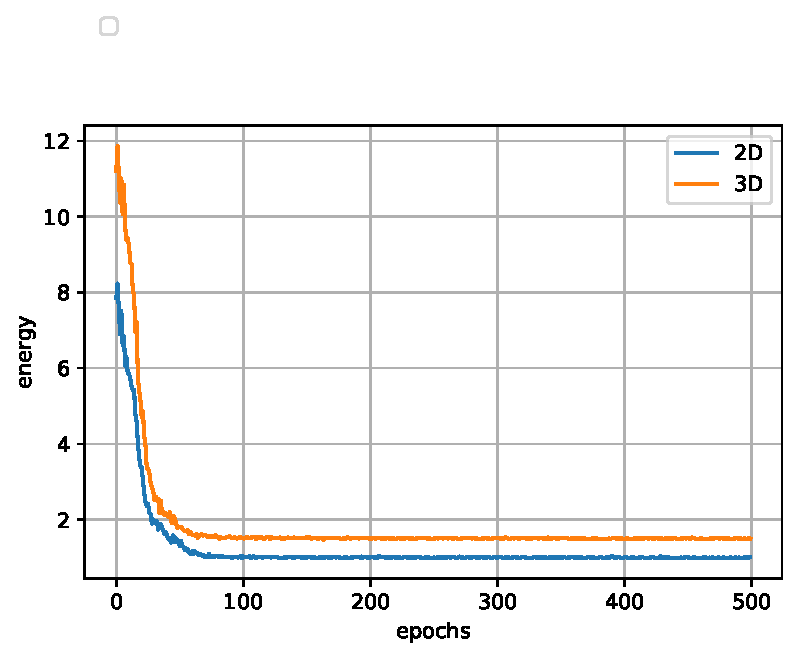
\includegraphics[]{figures/one_part_training2.pdf}
	\caption{Energy estimated from each batch during training of the DNN model on one particle in harmonic oscillator, in $2D$ and $3D$, respectively}
	\label{fig:one_part_training2}
\end{figure}

The minimization of $\langle E \rangle$ during training of the DNN model on one particle in 2D and 3D harmonic oscillator can be seen in \autoref{fig:one_part_training1}. Both energies approach the correct ground state energy, respectively $E=1$ and $E=1.5$ in two and three dimensions. Note also that towards the end of training, the fluctuations in the estimated energies die down. This is an indication that the trial wave function approaches the correct ground state, as $\sigma^2 = 0$ when $\psi_{Trial} = \psi_{GS}$.  


\begin{figure}[H]
	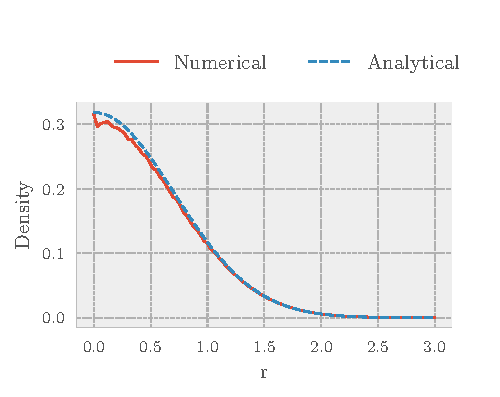
\includegraphics[]{figures/one_part_2D_dens.pdf}
	\caption{Radial one-body density for one particle in 2D harmonic oscillator. The density was calculated using $N=1e6$ samples from the trained DNN model, using $100$ bins on the interval $[0,3]$. It is compared to the analytical result}
	\label{fig:one_part_2D_dens}
\end{figure}

\begin{figure}[H]
	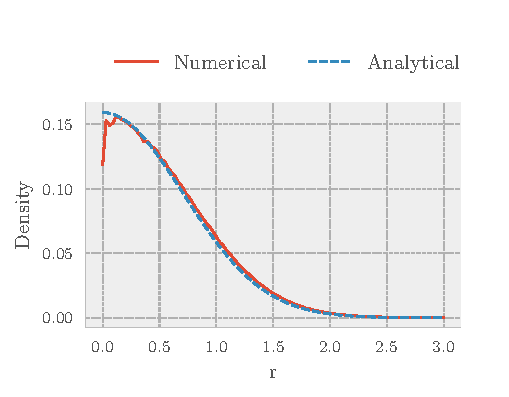
\includegraphics[]{figures/one_part_3D_dens.pdf}
	\caption{Radial one-body density for one particle in 3D harmonic oscillator. The density was calculated using $N=1e6$ samples from the trained DNN model, using $100$ bins on the interval $[0,3]$. It is compared to the analytical result}
	\label{fig:one_part_3D_dens}
\end{figure}

After the previous training, the radial one-body density is calculated using $N=1e6$ samples generated by the model. The densities are presented in \autoref{fig:one_part_2D_dens} and \autoref{fig:one_part_3D_dens}. Although the approximation is not as close as seen in \autoref{fig:one_part_func}, it is still fairly good. 

\subsubsection{Ground State Energies}

\begin{table}[ht]
	\begin{tabular}{r|rr}
		\toprule
		           & Numerical & Analytical \\
		1D, Tanh   & 0.5015(2) &   0.5      \\
		1D, ReLu   & 0.0032(2) &   0.5      \\
		2D, Tanh   & 1.0015(1) &   1        \\
		3D, Tanh   & 1.5046(1) &   1.5      \\
		\bottomrule
	\end{tabular}
	\caption{Summary of the estimated ground state energies of the DNN model trained on the previously discussed systems. The energy was estimated using $N=1e6$ samples}
	\label{tab:1}
\end{table}

In \autoref{tab:1}, a summary of the estimated ground stated energies of the DNN model trained on the previously discussed systems is presented. Without too much concern for choice of parameters, such as batch size, number of metropolis steps, or network architecture, all models but the Relu model produces results to accurate to $1\%-3\%$.


\subsection{RNN-DNN Hybrid Model for Non-Interacting Bosonic Quantum Dots}
\begin{figure}[H]
	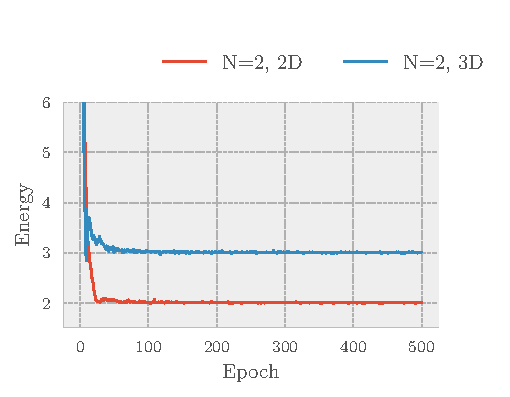
\includegraphics[]{figures/many_part_nonint_training1.pdf}
	\caption{Estimate of energy during training of RNN-DNN hybrid models. The models were trained on two non-interacting bosons in 2D and 3D harmonic oscillator. The models were trained for 1000 epochs, using a batch size of 500.}
	\label{fig:many_part_nonint_training1}
\end{figure}

\begin{figure}[H]
	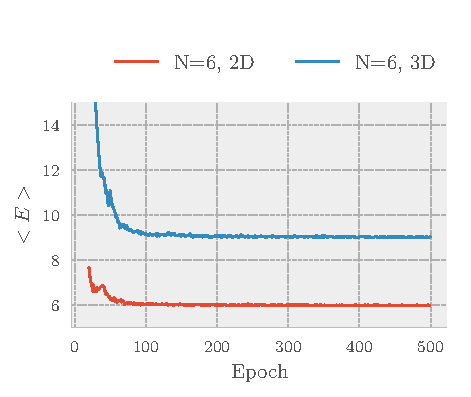
\includegraphics[]{figures/many_part_nonint_training2.pdf}
	\caption{Estimate of energy during training of RNN-DNN hybrid models. The models were trained on six non-interacting bosons in 2D and 3D harmonic oscillator. The models were trained for 1000 epochs, using a batch size of 500.}
	\label{fig:many_part_nonint_training2}
\end{figure}

In \autoref{fig:many_part_nonint_training1} and \autoref{fig:many_part_nonint_training2}, we see the minimization of energy as the RNN-DNN model is trained on various numbers of non-interacting bosons in 2D and 3D harmonic oscillators. In all cases, the model used a hidden state of 5 units, together with a two layer network with 32 nodes each. Although the RNN-DNN uses the hidden state to encode the correlation with previously sampled particles, it has no problem learning the ground state of uncorrelated systems, as seen in the figures. Note that in  \autoref{fig:many_part_nonint_training2}, a sudden dip in the energy in the beginning training can be seen for $N=6$ in 3D. This dip violates the variational principle. As nothing was done to regularize the trial wave function, it is perhaps unnormalizable during early stages of training, since the initial parameters are random. This will likely cause the metropolis algorithm to fail, as it is not possible to sample from such a distribution. Nevertheless, the model approaches the correct ground state energy.

\begin{table}[ht]
	\begin{tabular}{r|rr}
		\toprule
		& Numerical& Analytical     \\
		N=2, 2D    & 2.0017(5) &  2 \\
		N=6, 2D    & 6.0044(8) &  6 \\
		N=2, 3D    & 3.0021(5) &  3 \\
		N=6, 3D    & 9.012(1)  &  9 \\
		\bottomrule
	\end{tabular}
	\caption{Summary of the estimated ground state energies of the RNN-DNN model in the non-interacting case. The energy was estimated using $N=1e5$ samples}
	\label{tab:2}
\end{table}

From \autoref{tab:2}, we see that the RNN-DNN model attains good accuracy for the non-interacting case, both in 2D and 3D, averaging a relative error of $0.1\%$.

\subsection{RNN-DNN Model for Two Interacting Bosonic in 1D Quantum Dots}
\subsubsection{Training}

\begin{figure}[H]
	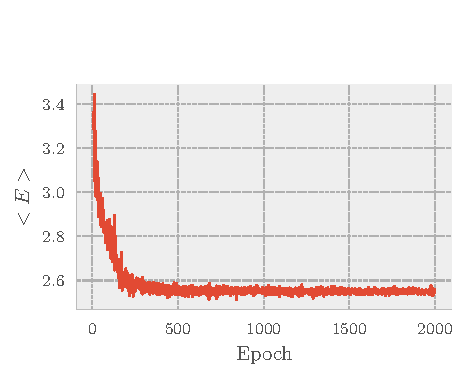
\includegraphics[]{figures/many_part_int_training1.pdf}
	\caption{Estimate of energy during training of RNN-DNN hybrid model. The model was trained on two interacting bosons in 1D harmonic oscillator. For the Coloumb interaction, a strength value of $\alpha = 1$ and a shielding value of $\beta 0.1$ was used. The models were trained for 2000 epochs, using a batch size of 2000.}
	\label{fig:many_part_int_training1}
\end{figure}

In \autoref{fig:many_part_int_training1}, we see the training process of two interacting bosons in 1D harmonic oscillator. The minimization of the energy is a bit more noisy than the previous non-interacting cases, hence the batch size was increased. The model used a hidden state of 5 units, together with a two layer network with 64 and 32 nodes, respectively.

Using $N=1e6$ samples, the ground state energy was estimated to be $E = 2.552(1)$. Compared to $E = 2.5482$ CISD energy using 40 orbitals(courtesy Øyvind Schøyen), the relative error is about $0.1\%$.

\subsubsection{One-Body Density}

\begin{figure}[H]
	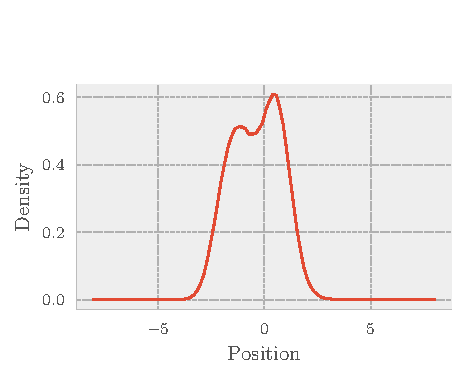
\includegraphics[]{figures/many_part_int_onebody.pdf}
	\caption{One-body density for two interacting bosons in 1D harmonic oscillator. The density was calculated using $N=4e5$ samples and $100$ bins on the interval $[-8,8]$.}
	\label{fig:many_part_int_onebody}
\end{figure}

\begin{figure}[H]
	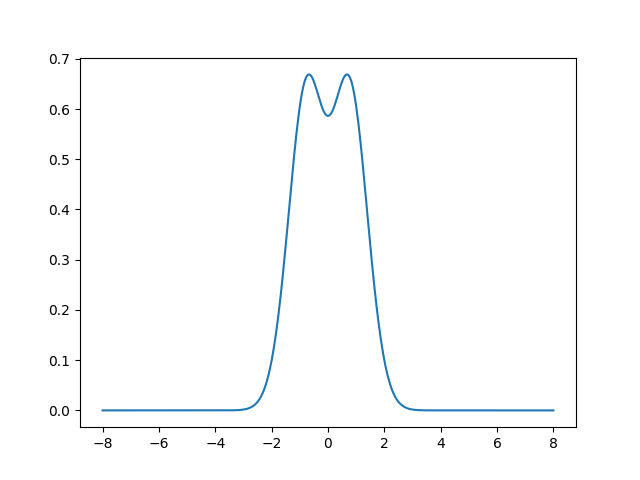
\includegraphics[scale = 0.4]{figures/oyvind.png}
	\caption{One-body density for two interacting bosons in 1D harmonic oscillator using CISD,courtesy Øyvind Schøyen}
	\label{fig:many_part_int_onebody}
\end{figure}

\autoref{fig:many_part_int_onebody} shows the corresponding one body density, which shows the characteristic separation of two peaks caused by the repulsive interaction. Comparing with the one-body density produced with the CISD simulation, the peaks are not as sharply defined. In terms of ground state energy, the RNN-DNN model successfully accounts for the correlation of the system, showing that the hidden state is able to encode the correlation in a meaningful way. However, like other approches in machine learning VMC, such as RBM, it struggles to reproduce the correct one-body density. 

\subsubsection{Conditional Probabilities}

\begin{figure}[H]
	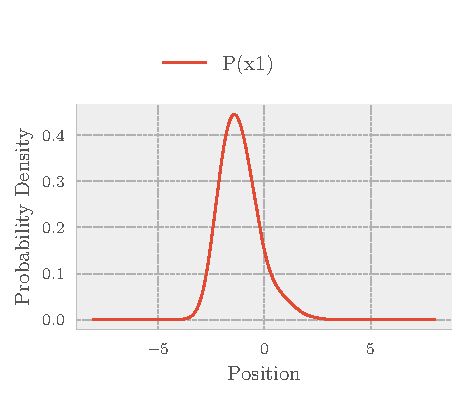
\includegraphics[]{figures/many_part_con1.pdf}
	\caption{One-body density for two interacting bosons in 1D harmonic oscillator. The density was calculated using $N=4e5$ samples and $100$ bins on the interval $[-8,8]$.}
	\label{fig:many_part_con1}
\end{figure}

\begin{figure}[H]
	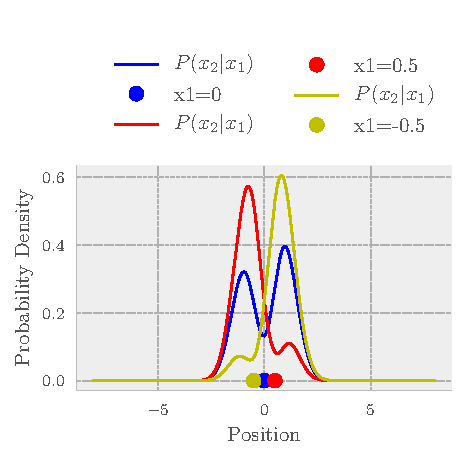
\includegraphics[]{figures/many_part_con2.pdf}
	\caption{One-body density for two interacting bosons in 1D harmonic oscillator. The density was calculated using $N=4e5$ samples and $100$ bins on the interval $[-8,8]$.}
	\label{fig:many_part_con2}
\end{figure}

In \autoref{fig:many_part_con1} and \autoref{fig:many_part_con2}, we see the conditional probabilities produced by the RNN-DNN model trained on two interacting bosons in 1D harmonic oscillator. In \autoref{fig:many_part_con1}, we see that the probability density for particle 1 is skewed towards the left. As there is no physical reason for why the first sampled particle is found more often to the left, one should think of the conditional probabilities more as rules for sampling the particles, rather than physical objects. In fact, given $P(x_1, x_2)$, there is no unique way of factoring it to conditional probabilities: 
\begin{align*}
	P(x_1, x_2) = P(x_1)P(x_2|x_1) =\\
	f(x_1)P(x_1)\frac{P(x_2|x_1)}{f(x_1)} = \tilde{P}(x_1)\tilde{P}(x_2|x_1),
\end{align*}
where $f(x_1)$ is an arbitrary function.

In \autoref{fig:many_part_con2}, we see however that some physical meaning is retained. The probability density of particle two conditioned on particles one's position act as to avoid particle one. Given particle one's position, the probability of sampling particle two's position close to it is relatively small compared to sampling it further away. This is a reflection of the repulsive potential, which pushes the particles appart.
 
\subsubsection{Sampling from Conditional Probabilities}
Next, we inspect if using Bruteforce Metropolis to sample from distributions produce densities that are faithful to that distribution.

\begin{figure}[H]
	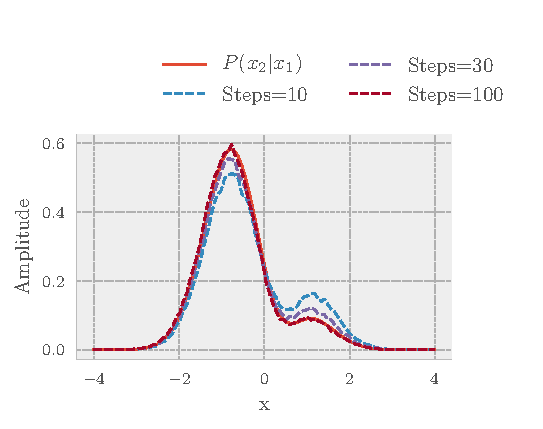
\includegraphics[]{figures/many_part_met.pdf}
	\caption{One-body density for two interacting bosons in 1D harmonic oscillator. The density was calculated using $N=4e5$ samples and $100$ bins on the interval $[-8,8]$.}
	\label{fig:many_part_met}
\end{figure}

In \autoref{fig:many_part_met}, the target probability density is $P(x_2|x_1=0.5)$ produced by the RNN-DNN model trained on the system as previously discussed. The densities were estimated using Bruteforce Metropolis with a step length of $1$ and va varying number of thermalization steps. For a low number of steps, such as $10$, it can be seen from the figure that the estimated density does not match the one produced by the model. Since the random walkers start off uniformly, they need a sufficient amount of steps so that they don't end up getting stuck in low probability areas, as seen to the left in the figure. If this happens, we fail to sample variables that are distributed as our model dictates. From the figure, we see that a increased number of steps remedy this.  

\subsection{RNN-DNN Model for Two Interacting Bosonic In Higher Dimension}

\subsubsection{Ground Sate Energy}

\begin{table}[ht]
	\begin{tabular}{r|rr}
		\toprule
		      & RNN-DNN   & DMC     \\
		2D    & 3.014(3)  &  3.00000(1) \\
		3D    & 3.751(1)  &   3.730123(3) \\
		\bottomrule
	\end{tabular}
	\caption{Estimated ground state energies of the RNN-DNN model train on two interacting bosons in 2D and 3D harmonic oscillator, respectively. In both cases, 10 hidden units and two layers of 64 and 32 nodes were used. The batch size was 4000 and the models were trained for 1000 epochs. The energy was estimated using $N=1e5$ samples.}
	\label{tab:3}
\end{table}

From \autoref{tab:3}, we see the estimated ground state energy of the RNN-DNN model trained on two interacting bosons in 2D and 3D harmonic oscillator. Taking the DMC calculation as ground truth, the numerical error is under $1\%$ in 2D and 3D, as with the 1D case. 

\subsubsection{One-Body Density}
\begin{figure}[H]
	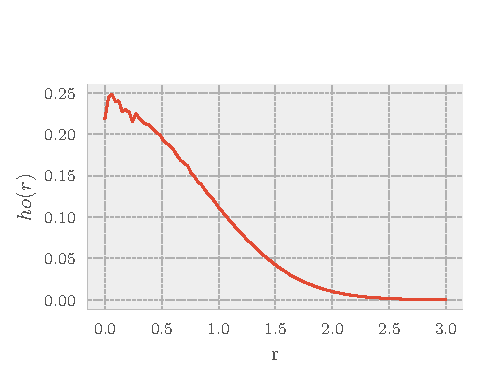
\includegraphics[]{figures/many_part_3D.pdf}
	\caption{One-body density for two interacting bosons in 1D harmonic oscillator. The density was calculated using $N=4e5$ samples and $100$ bins on the interval $[-8,8]$.}
	\label{fig:many_part_3D}
\end{figure}

\begin{figure}[H]
	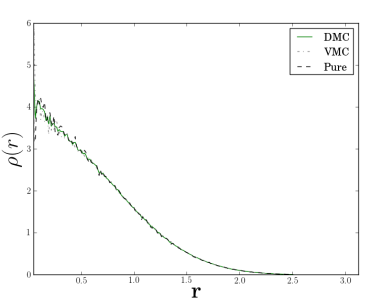
\includegraphics[scale=0.6]{figures/onebody3d.png}
	\caption{One-body density for two interacting bosons in 1D harmonic oscillator. The density was calculated using $N=4e5$ samples and $100$ bins on the interval $[-8,8]$.}
	\label{fig:many_part_DMC}
\end{figure}

In \autoref{fig:many_part_3D} and \autoref{fig:many_part_DMC} we see the radial one-body density of two interacting bosons in 3D harmonic oscillator calculated using our RNN-DNN model and DMC, respectably. Note that technically, the DMC calculation was performed on a two electron system, but since this state is symmetrical with respect to spatial coordinates, it is comparable to our bosonic system. In addition, the density is not scaled.

Since the figures are produced independently, they are hard to compare. However, some general features can be seen: 1/3 of the max amplitude occur around $r=1$, and the density have almost completely diminished around $r=2$. On the other hand, the density produced by the RNN-DNN model is not as linear towards the origin as the DMC density, again indicating the our model may struggle reproducing the correct one-body density.


%%% Local Variables:
%%% mode: latex
%%% TeX-master: "../main"
%%% End:
